\chapter{GUI dell'app}

\section{Avvio dell'app}

Quando si avvia l'app viene visualizzato un avviso che invita l'utente a premere sul bottone in basso a destra per far partire la scansione dei dispositivi BT.

\begin{figure}[ph]
	\centering
	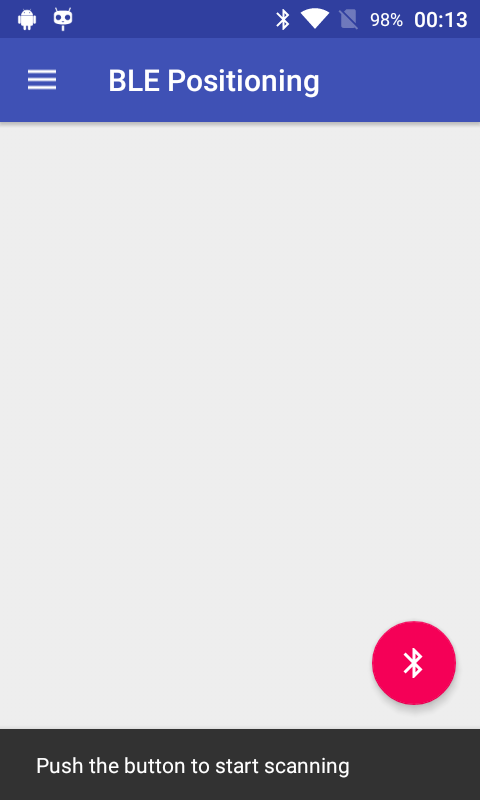
\includegraphics[width=.35\linewidth]{img/app/01.png}
	\caption{Avvio dell'app}
\end{figure}

\newpage
\section{Abilitazione della radio Bluetooth}

Questa schermata viene visualizzata se la radio BT è spenta. Appare all'avvio dell'app o di una nuova scansione.
\begin{figure}[ph]
	\centering
	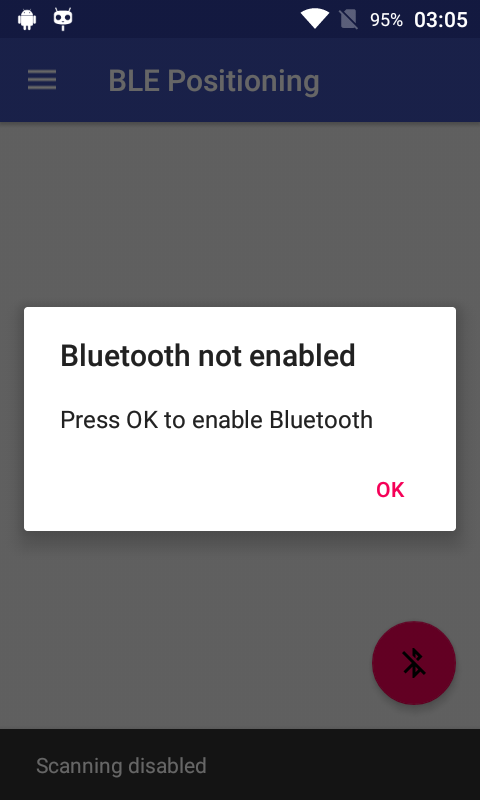
\includegraphics[width=.35\linewidth]{img/app/17.png}
	\caption{Abilitazione della radio Bluetooth}
\end{figure}

\newpage
\section{Scansione dei dispositivi}

In questo fragment viene caricata la RecycleView con i dati dei dispositivi. Questa lista può essere ordinata in base ai settaggi scelti. Se si seleziona un dispositivo vengono visualizzati i relativi dettagli.

\begin{figure}[ph]
	\centering
	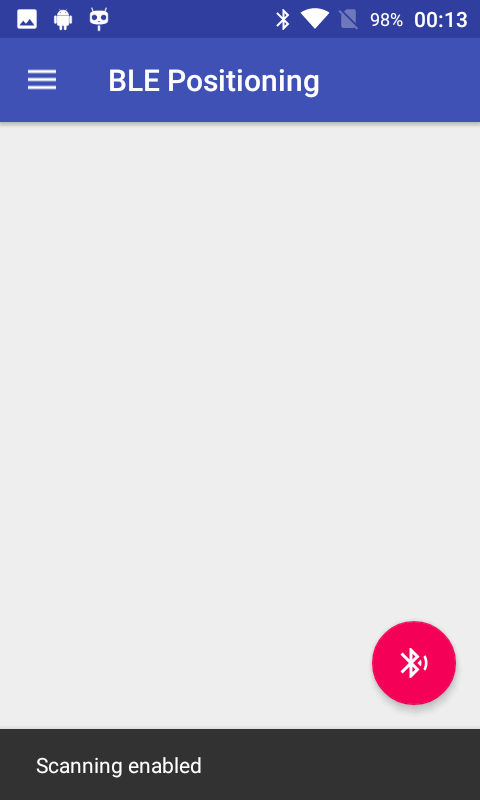
\includegraphics[width=.35\linewidth]{img/app/02.png}
	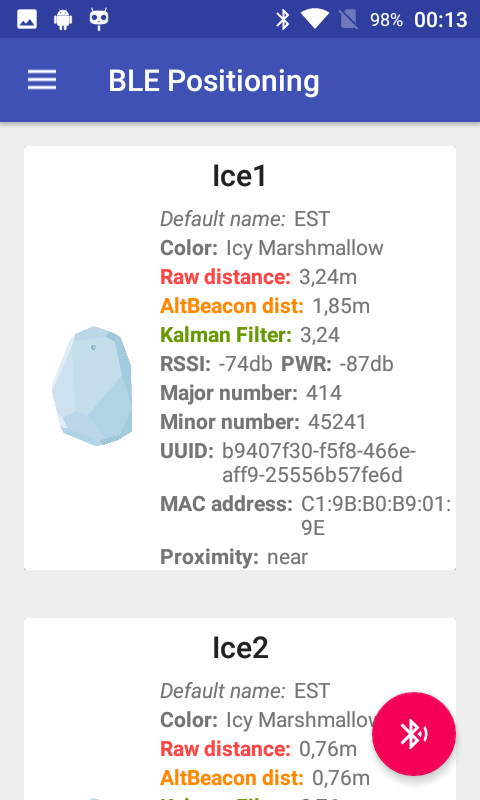
\includegraphics[width=.35\linewidth]{img/app/03.png}
	\caption{Scansione dei dispositivi}
\end{figure}

\newpage
\section{Menù a sinistra}

In questo menù viene data la possibilità di tarare la distanza con Arduino (campo Measurement), visualizzare i settings oppure ritornare alla vista principale.
\begin{figure}[ph]
	\centering
	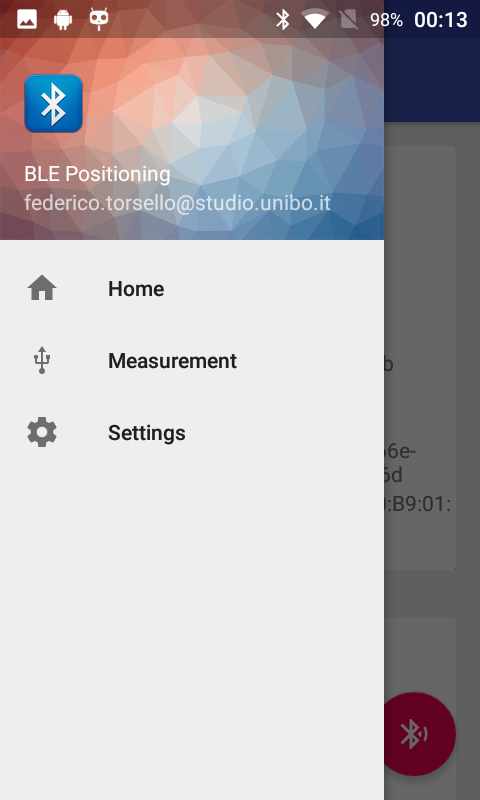
\includegraphics[width=.35\linewidth]{img/app/04.png}
	\caption{Menù a sinistra}
\end{figure}

\newpage
\section{Menù a destra}

Il menù a destra consiste in un fragment in cui l'utente può selezionare le proprie preferenze. Nel caso in cui la scansione fosse interrotta, i settaggi risultano non abilitati.

\begin{figure}[ph]
	\centering
	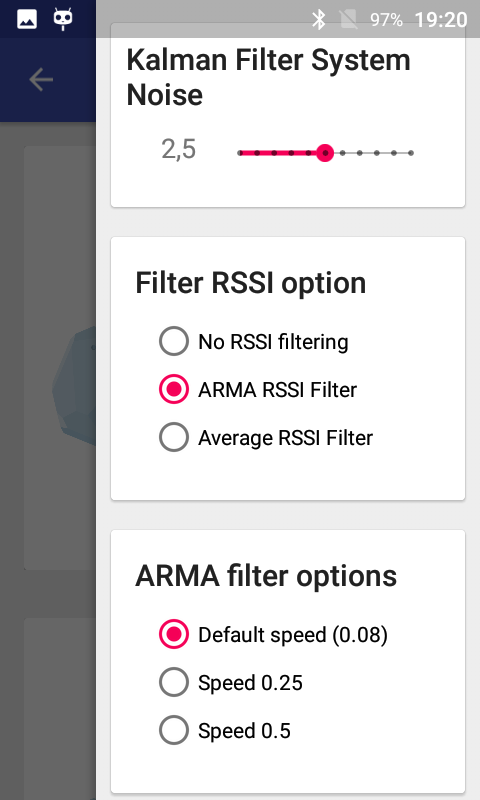
\includegraphics[width=.35\linewidth]{img/app/08.png}
	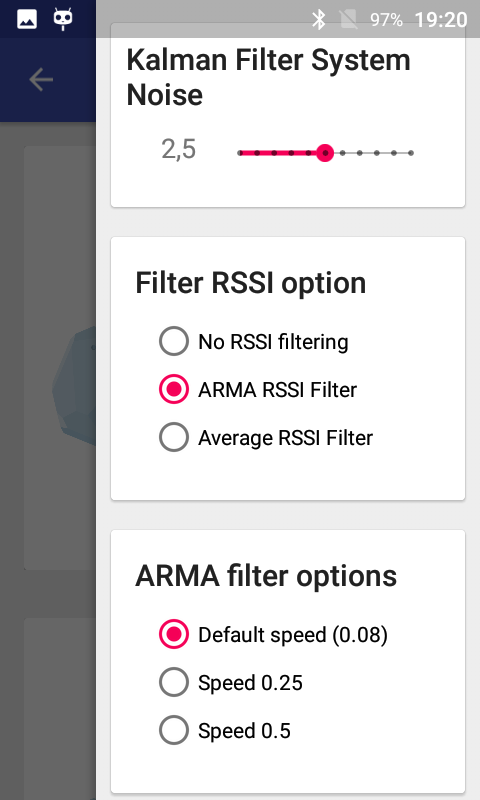
\includegraphics[width=.35\linewidth]{img/app/05.png}
	\\
	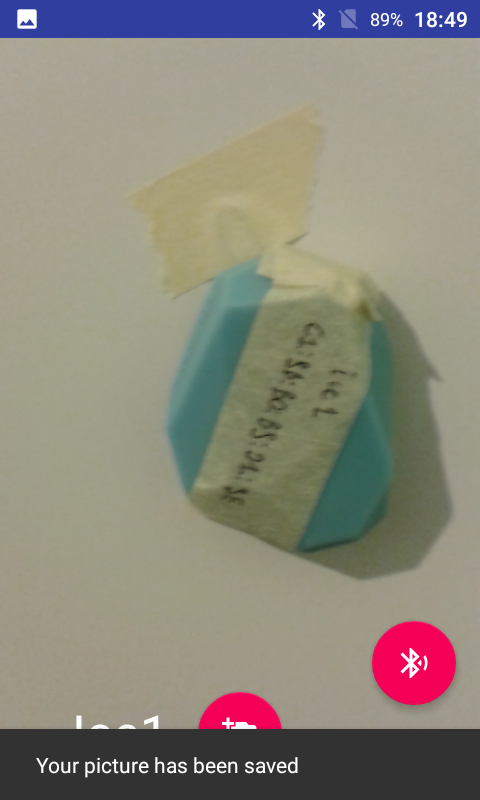
\includegraphics[width=.35\linewidth]{img/app/07.png}
	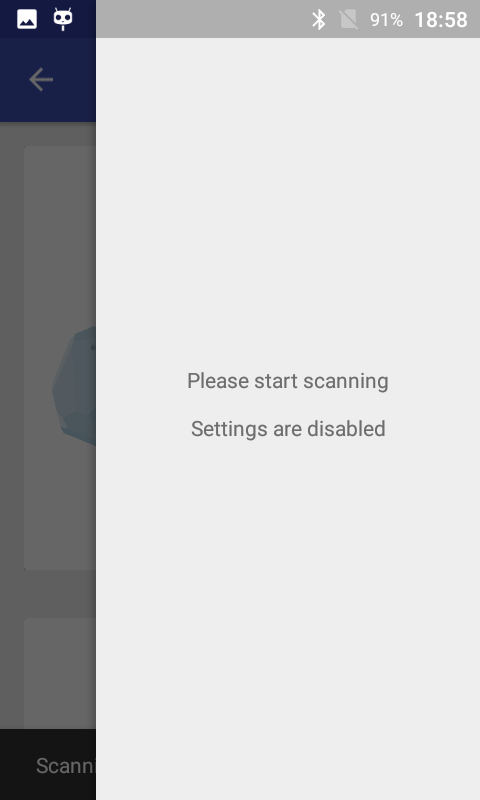
\includegraphics[width=.35\linewidth]{img/app/06.png}
	\caption{Menù a destra}
\end{figure}

\newpage
\section{Foto ad un dispositivo}
Possibilità di scattare una foto a un dispositivo BT per ricordare dove è stato posizionato.
\begin{figure}[ph]
	\centering
	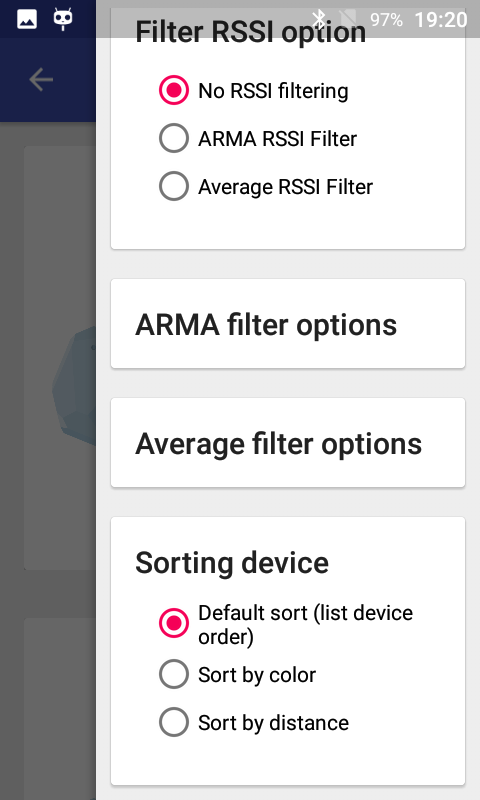
\includegraphics[width=.35\linewidth]{img/app/15.png}
	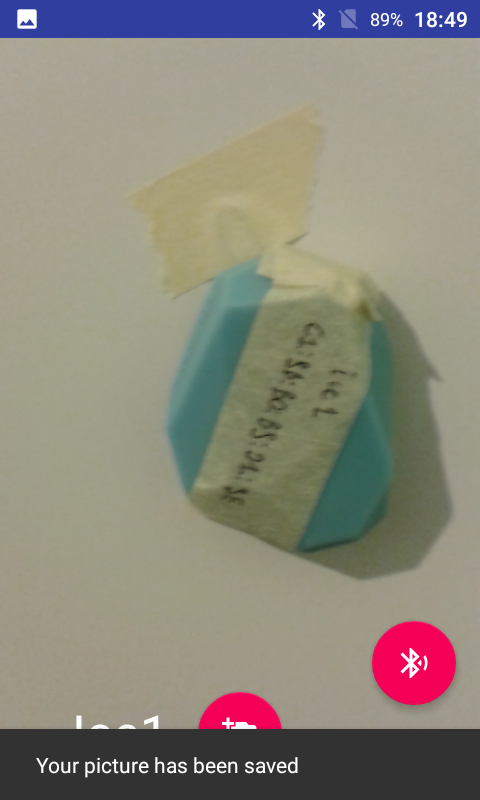
\includegraphics[width=.35\linewidth]{img/app/16.png}
	\caption{Foto ad un dispositivo}
\end{figure}

\newpage
\section{Dettagli dei dispositivi}
Il fragment dei dettagli è diviso in tre parti: Testing, \textit{fragment centrale} e Real time charts.  In tutte le parti si è riportata la stima con Arduino come riferimento reale.

\begin{itemize}
	\item \textbf{Testing}: sezione in cui si registrano dati sulla stima e si creano report.
	\item \textbf{Fragment centrale}: sezione che riporta i dettagli del dispositivo selezionato. Il nome del fragment (ad esempio Ice1) deriva dal dispositivo scelto.
	\item \textbf{Real time charts}: sezione in cui sono riportati più grafici real time al fine di visualizzare le varie stime sulla distanza.
\end{itemize}

\begin{figure}[ph]
	\centering
	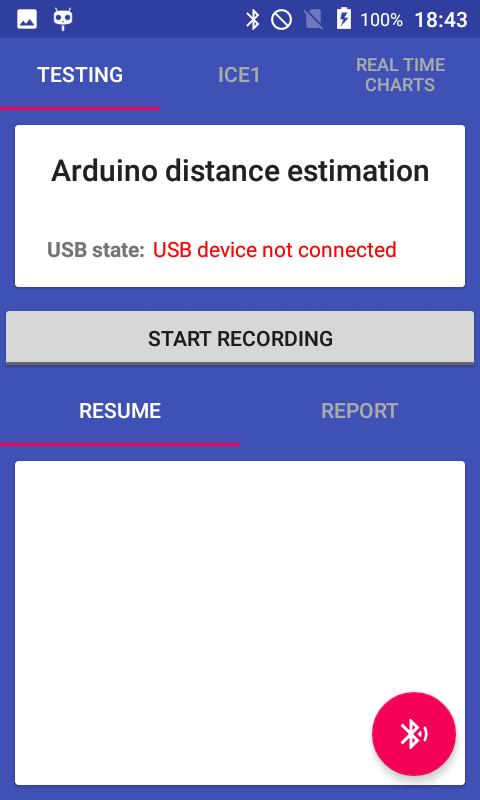
\includegraphics[width=.32\linewidth]{img/app/11.png}
	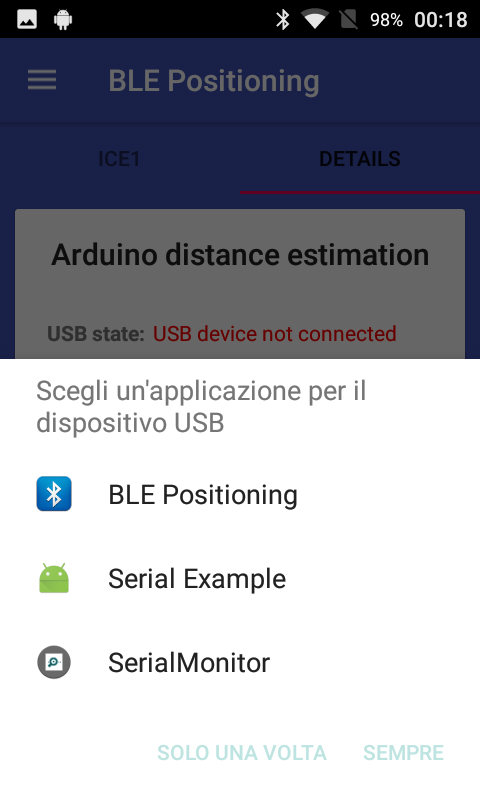
\includegraphics[width=.32\linewidth]{img/app/09.png}
	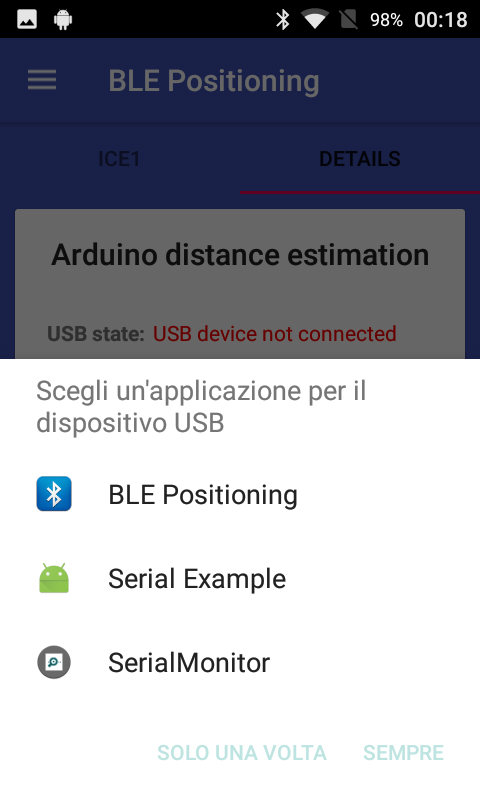
\includegraphics[width=.32\linewidth]{img/app/10.png}
	\caption{Dettagli, testing e grafici real time}
\end{figure}

\newpage
\section{Testing fragment}
Per poter eseguire il testing è stato aggiunto un fragment con due fragment child (\textit{Resum} e \textit{Report}) ed un button. Premendo il button si avvia la registrazione di 5 secondi dei dati sulla stima della distanza. Una volta registrati, questi dati vengono salvati sul dispositivo in un file \textit{.txt} e \textit{.json} e visualizzati nelle sopracitate schede.
\begin{figure}[ph]
	\centering
	
	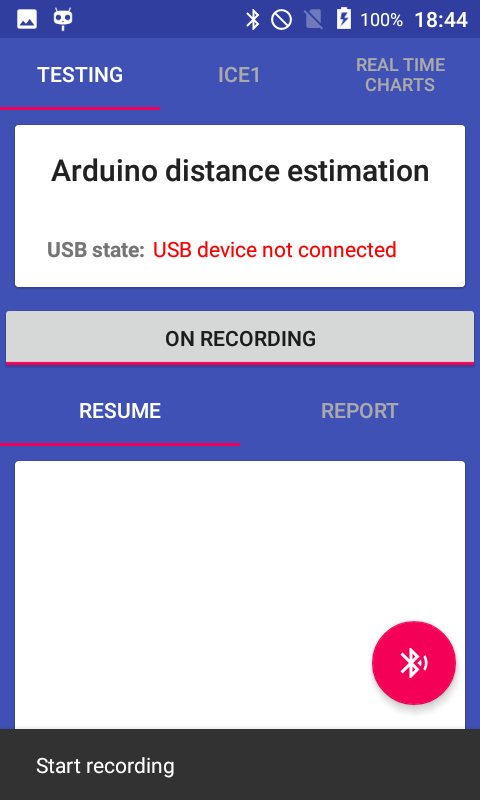
\includegraphics[width=.32\linewidth]{img/app/12.png}
	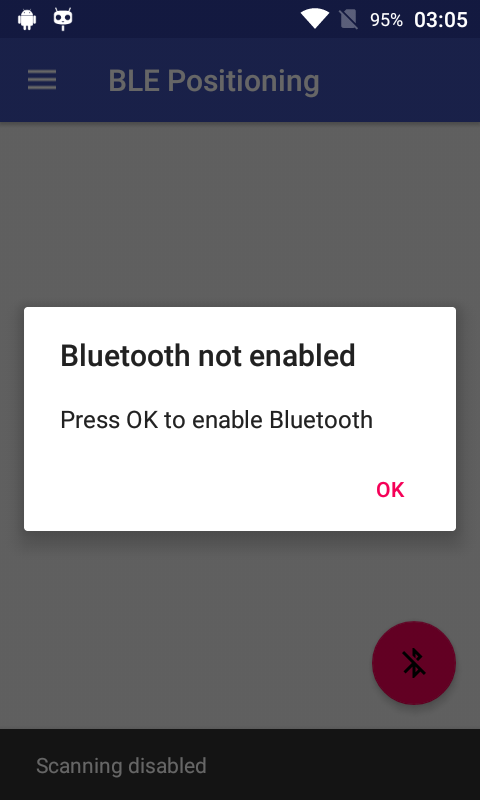
\includegraphics[width=.32\linewidth]{img/app/13.png}
	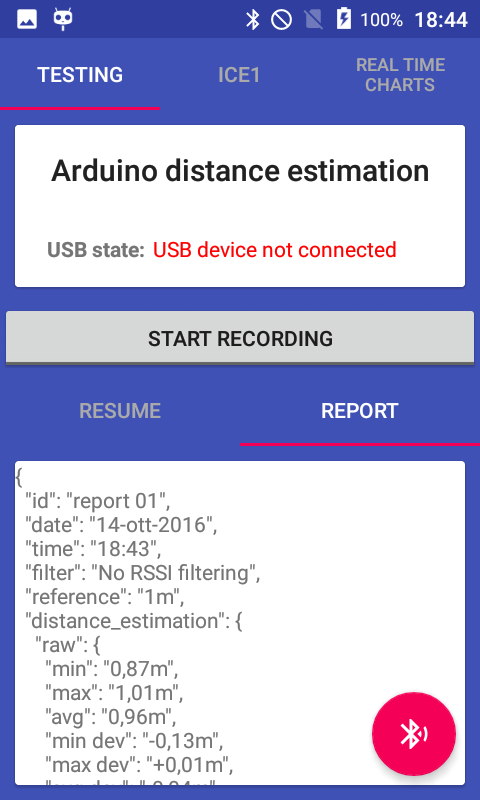
\includegraphics[width=.32\linewidth]{img/app/14.png}
	\caption{Testing, resume e report in app}
\end{figure}

\newpage
\section{Connessione con Arduino via USB OTG}
Con questi messaggi si richiede all'utente di abilitare la comunicazione USB sul dispositivo. Senza questa abilitazione la comunicazione con l'Arduino non può avvenire.
\begin{figure}[ph]
	\centering
	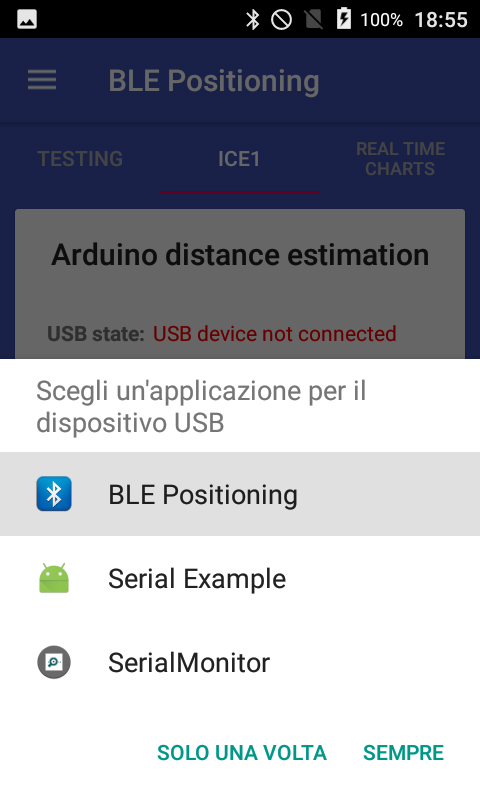
\includegraphics[width=.35\linewidth]{img/app/18.png}
	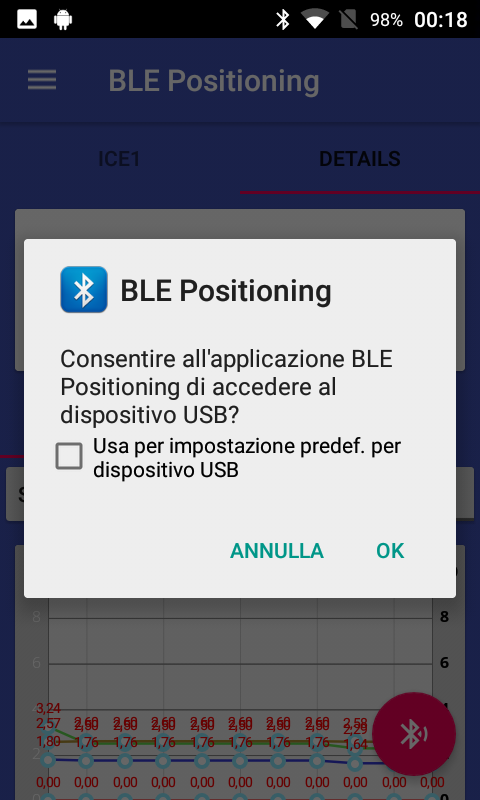
\includegraphics[width=.35\linewidth]{img/app/19.png}
	\caption{Connessione con Arduino via USB OTG}
\end{figure}

\newpage
\section{Feedback della stima della distanza con Arduino}
In questo fragment si visualizza la stima della distanza con Arduino quando il cavo è connesso e la comunicazione USB con OTG è abilitata.
\begin{figure}[ph]
	\centering
	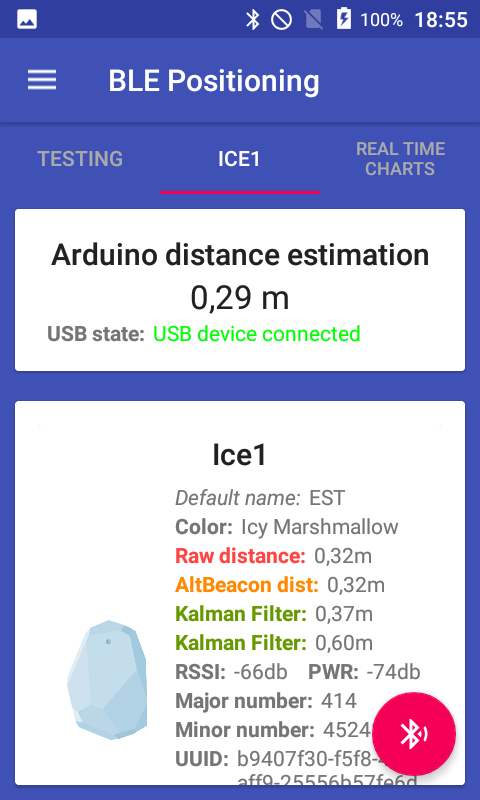
\includegraphics[width=.35\linewidth]{img/app/20.png}
	\caption{Feedback della stima della distanza con Arduino}
\end{figure}

